
\textbf{\huge{Résumé}}\\[1cm]
\begin{center}
Certaines pathologies visuelles, principalement d'origine dégénérative, sont incurables. Ils conduisent souvent à une déficience visuelle, parfois à la cécité. Cette déficience visuelle
handicape la personne dans toute sa vie en diminuant son efficacité dans ses activités quotidiennes, en augmentant les risques de chutes ou d'accidents, en la coupant petit à petit
de toute vie sociale, culturelle et parfois même familiale... au problème de la vision, s'ajoute donc un véritable problème humain.
Face à ce constat, notre projet a développé des lunettes intelligentes pour malvoyants dont le principe est d'aider la personne malvoyante à entendre ce qu'elle veut voir. En d'autres termes, ces lunettes intelligentes convertiront le contenu d'une image ou d'une vidéo en un fichier audio. 
\\[1cm]
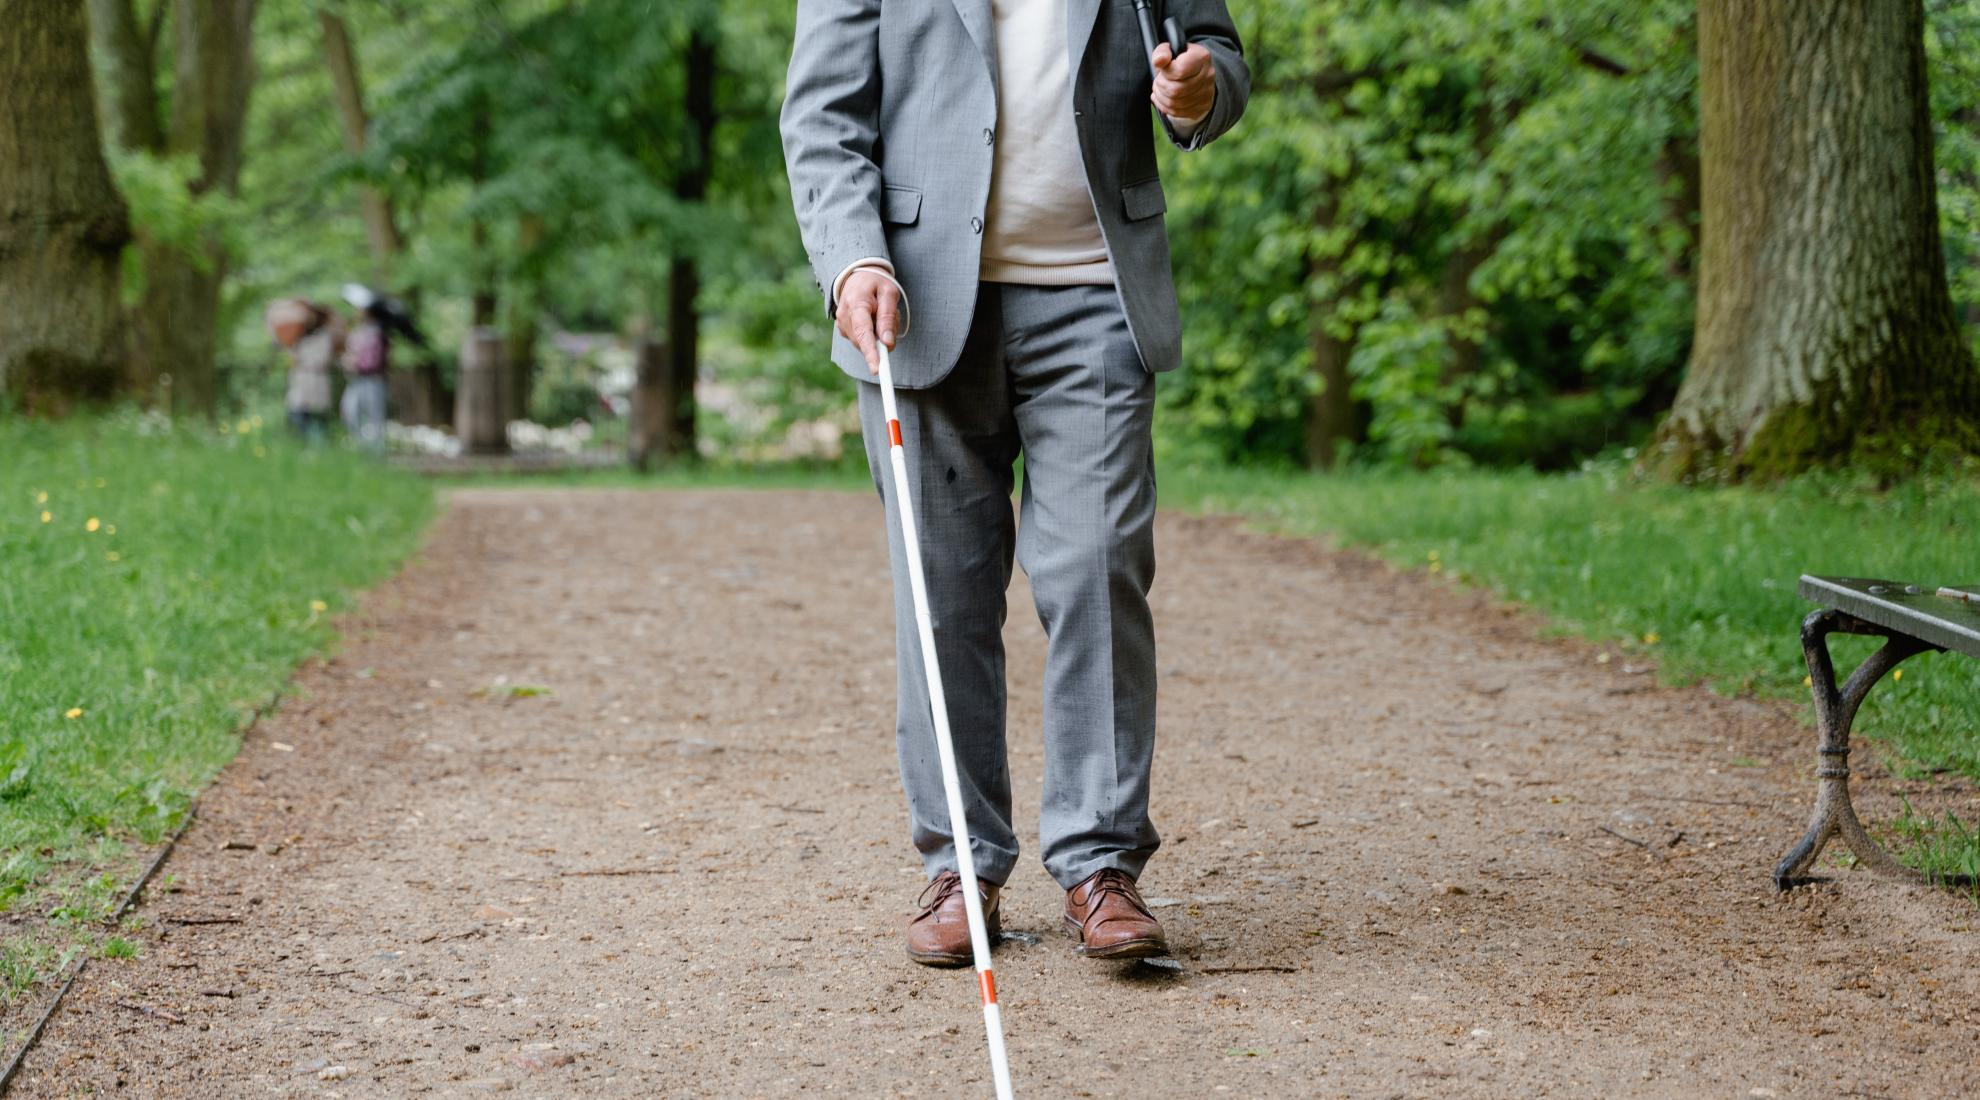
\includegraphics[width=14cm, height=7cm]{4-Images/visually-impaired.jpeg}\\[2cm]

\end{center}
